%*******************************************************************************
%*********************************** First Chapter *****************************
%*******************************************************************************

\chapter{Introduction}  %Title of the First Chapter 
\label{chap:Intro}

\graphicspath{{Chapter1/Figures/} {Chapter1/Figures}}
\begin{quote}
%\textsl{One should never try to prove anything that is not almost obvious - Alexander Grothendieck}
\textsl{There are things known and there are things unknown, and in between are the doors of perception} - Aldous Huxley - \textsl{Doors of perception}
\end{quote}


\section{Introduction}

We live in a world where information is being bombarded on our cognitive faculties from all sides, at all times. The internet is a continuous stream of information and each source is fighting with the other to get a piece of our attention budget. 
With the advent of machine learning and big-data sources, building systems that predict actions as a response to perceptual triggers is the bread and butter of many companies. The use cases may range from understanding which advertise made a visitor do an unscheduled purchases on amazon, or which string of music tracks recommendations maximized a users time on a particular music platform. But in the end it all boils down to understanding what triggers result in human action or lack there of~\cite{song2012survey}. Nonetheless the systems that surrounds a human interacting with the internet, are all figuring out the best triggers which are perceived by the human as worthy of attention. 
The term ``Attention Economy''~\cite{davenport2001attention} was actually coined for this very reason. In the words of Matthew Crawford ``\textit{Attention is a resource, a person has only so much of it.}''~\cite{MatthewCrawford}. We live in the age of distraction, and more often than not, our subjective perceptions are guiding our actions, than our conscious cognitive processes. Several studies have shown that engagement is almost always a game of stimulating our most basic urges, such as dopamine hits, presence of faces or simply arousal of emotions to increase the working memory.~\cite{bakhshi2014faces,joglekar2017like}~\cite{schupp2006emotion}~\cite{soat2015social}. 


An interesting side effect of dwindling attention budgets is the emergence of more formal topical spaces on the internet. The ever pervasive nature of the internet allow these formal spaces to function almost like physical communities, with moderated and effective peer to peer exchange of thoughts, ideas and empathy~\cite{kummervold2002social,squire2015should,hwang2010social}.
In such an environment, as computer scientists, it is worth asking the questions:

\noindent\fbox{\begin{minipage}[t][2\height][c]{\dimexpr\textwidth-2\fboxsep-2\fboxrule\relax}
        \centering
        How do subjective human perceptions manifest in data?\\
        
        
        Can quantifying these help us design better interventions ?\\
        
\end{minipage}}

\vspace{1cm}
These two questions are going to be the guiding principles of my dissertation. But first of all, we need to clarify the relation between perception, affects and data. To do so we should try and understand each of these terms separately in the context of the field of application.

\section{Perception and Affect}
Across my work , I would try to build frameworks to capture subjective human perceptions in the realm of human to human interactions and subjective intangible qualities like the sense of beauty or the sense of perceived support. The utility of such an attempt, can only be justified if there is a real link between how humans function at the most fundamental cognitive level and how they perceive the intangible, including the aesthetic. There has been an ongoing effort to unravel this link, through psychological, neuro-evolutional and philosophical arguments. I will try to gain inspiration from them, but a detailed critique is beyond the scope of my dissertation and expertise\\
\begin{definition}
    \textbf{Affect~\footnote{American Psychological Association definition.}}: Any experience of feeling or emotion, ranging from suffering to elation, from the simplest to the most complex sensations of feeling, and from the most normal to the most pathological emotional reactions.\\
\end{definition}


\begin{definition}
    \textbf{Perception~\footnote{American Psychological Association definition.}}: The process or result of becoming aware of objects, relationships, and events by means of the senses, which includes such activities as recognizing, observing, and discriminating. These activities enable organisms to organize and interpret the stimuli received into meaningful knowledge and to act in a coordinated manner.
\end{definition}


Emotions or `affects' and perceptions have long been discussed in the psychology, neuroscience and philosophical literature. Emanuel Kant in his prolific work, first discussed the utility and the philosophical reasoning behind presence of affects or emotions\cite{kant1987critique}. In his opinion, emotions are pre-cognitive involuntary states, termed as "mere perceptions of unspecified bodily states"\cite{borges2004can}. But that does not mean they don't influence our deepest level of well-being and influence our decision making processes.
The link between affect and perception has also been explored in several other cases. An argument to link perception of affect producing aesthetics was made by Perlovsky\cite{perlovsky2014aesthetic}, where they propose that the phenomenon of affects arousing from aesthetics, comes from a fundamental human need to enrich the knowledge about real world. An unexpected thing, stimuli or structure in physical space creates a dissonance between our expected model of the world and the perceived reality at some level and we perceive it as aesthetically pleasing. Another recent study by Zadra et.al\cite{zadra2011emotion} evaluated the relation between visual perception and emotions. They demonstrate that the conventional assumption of the disentangled functioning of perception and affects is not necessarily true. Humans are quite susceptible to perceiving different realities based on different aroused affects. 

The discussion on the formal definition and process of affects will continue, but there seems to be a consensus, at-least among the computer science and information science community that affects do influence our decisions and we perceive information through a filter of affects. Affective triggers can be generated when information is formatted or packaged in a certain way. In such a setup, it is worth testing if certain affect driven interactions on the web leave a trail of patterns in the data of these interactions. Furthermore it is work asking if these patterns might in some way be used to improve our online and physical environments. But to arrive at these patterns, one needs to understand the frameworks of approaching such a problem. The journey from Data to subjective signatures, has to go through a series of operations. 

\section{Intervention and the DIKW model}

\begin{figure*}[t!]
    \centering
    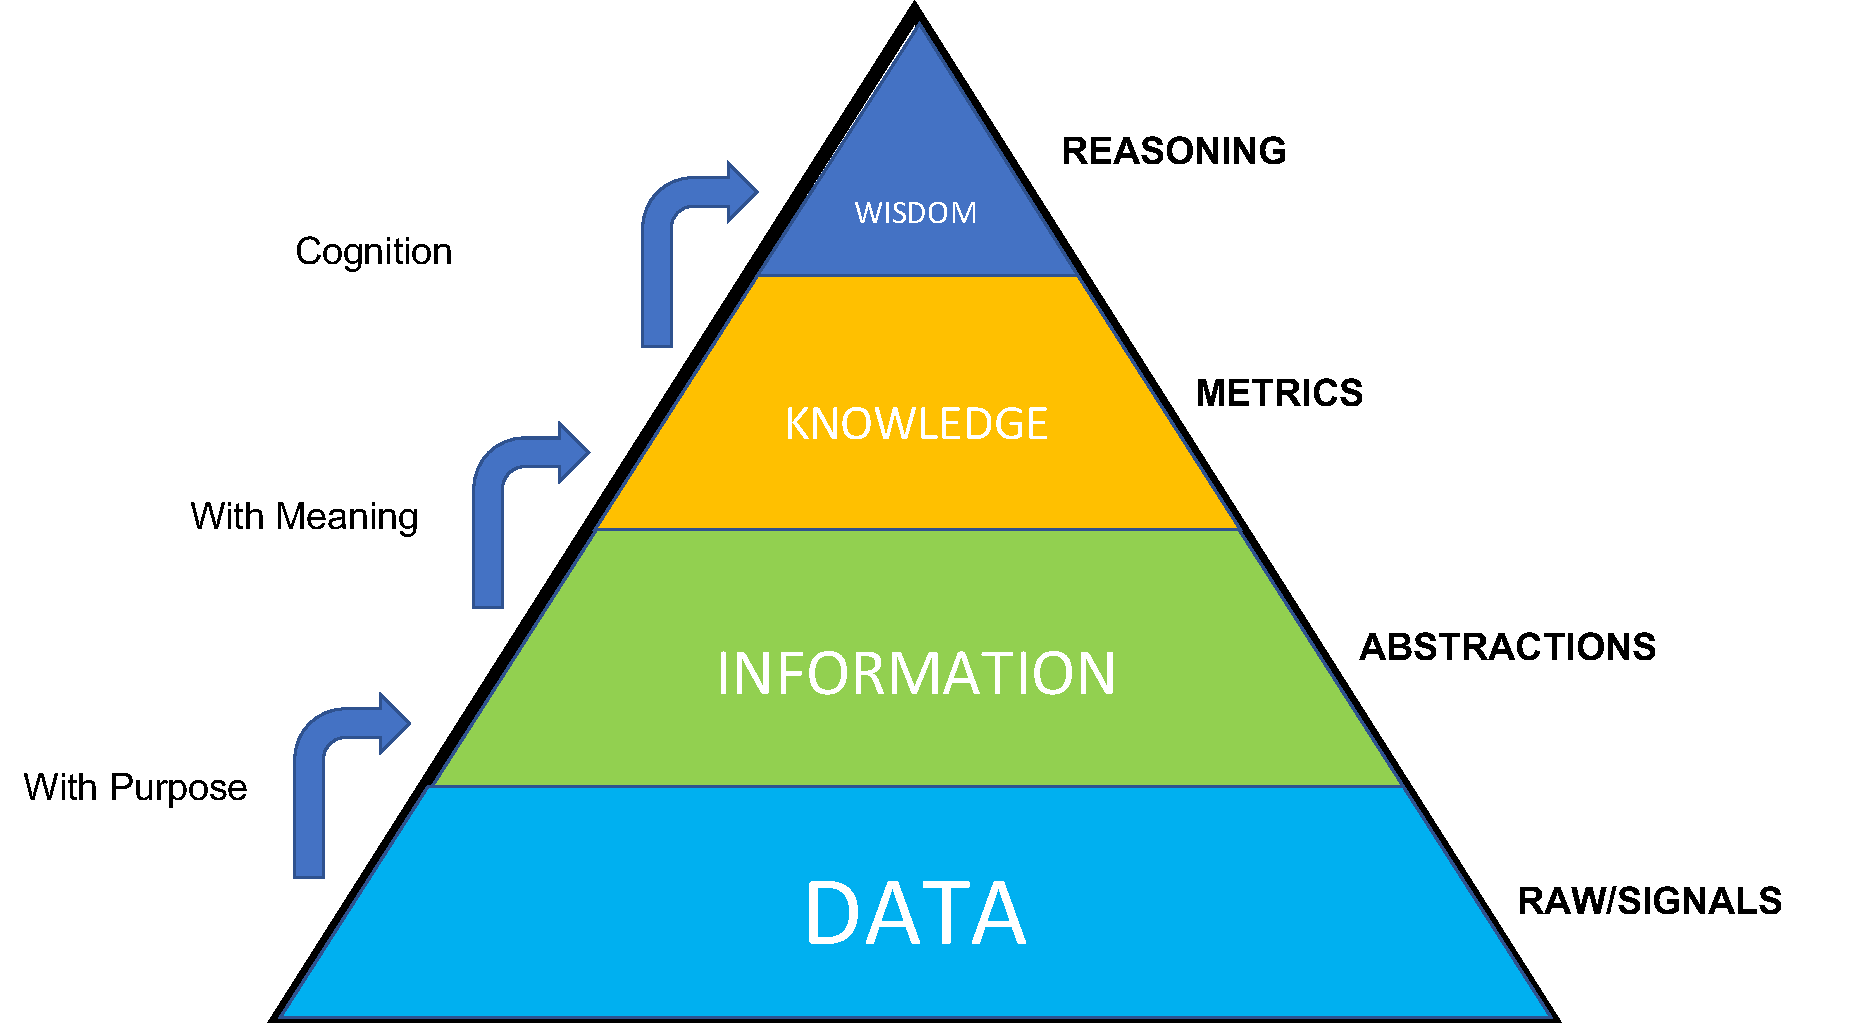
\includegraphics[width=\columnwidth]{DIKW.pdf}
    \caption{The DIKW pyramid}
    \label{fig:dikw}
\end{figure*}

In attempt to develop metrics and pipelines, one has to reflect on one of the fundamental frameworks about operations on data, that is the \textbf{Data , Information, Knowledge and Wisdom} model\cite{rowley2007wisdom}.In this dissertation I posit and demonstrate through case studies, that for any reasoning about subjective perceptions , you need to develop frameworks that extract knowledge from data in a format that is aligned with the ontological framework of the application. In the context of this dissertation, ontology implies a set of concepts, definitions and relations between entities defined around a common set of axioms. I show that if a set of relations and definitions of concepts in the area of intervention are present, `a' solution can be reached provided that systems are designed to interpret metrics extracted from the data in relation to the ontology of the area of application. But to reach this step, the data needs to pass through the 4 layers of the DIKW pyramid model.

In this model, the most foundational layer consists of the pure form raw \textbf{data or signals} that come from a source. If we are measuring subjective perceptions of humans, this source needs to be tied back to humans in some way. To that extent, the data must ideally be a product of human to human interaction online. Or it needs to capture the human perceived responses, through explicit exercises like crowd sourcing or public surveys. In this dissertation, I present various data sources and methods of collecting and curating data, which pertain to human-human interactions or human responses. 

The \textbf{information} layer is the result of the fact that any process done on the data is with a sense of purpose or an end goal. For example, if the goal is to understand how humans exchange messages at times of distress, you would most certainly need to express the raw information about sender and recipient of messages into some form of a networked abstraction. The abstraction preserves the organization of data, but at the same time allows information to be operated on. As a result, almost always the output of this process is some form of a data abstraction. You need to attach some meaning to the patterns in the information to extract knowledge about the fundamental processes that you want to measure.

\textbf{Knowledge}. Defining knowledge has been an ongoing effort in the field of philosophy. But in the context of information science, knowledge involves collation of diverse sources of information and  mix of contextual information, values and metrics to deliver a coherent understanding of the real world. For example, if you need to know the most popular user among a social network of users exchanging messages; you would look for the most central user in the network(abstraction) along with several other temporal and structural metrics to arrive at a few candidates. In this particular case, these metrics, along with the context of the social network's design, dawns the meaning of popularity. 

The final layer needs a cognitive process and an ontological framework, to extract actionable insights, which we can call \textbf{wisdom}. By classical definition of ontology, it defines properties of and relations between objects or concepts. For this very reason, these ontological frameworks need to be originating from the fields of intervention.  In our example, lets assume we need to get some insights about the dynamics of popular users. Particularly in the context of optimizing advertising delivery. For example we need to understand how a particular piece of advertising, might percolate through the network if certain popular users advertise it~\cite{li2012diffusion}. However , to arrive at these insights we need to be grounded in the ontological frameworks of epidemiology, network physics and depending on the application, advertising or meme theory. Then using the abstractions of social networks, the metrics derived from them, and the ontological basis of all the aforementioned fields, one can design a pipeline that could deliver us these insights with reasonable accuracy. 

Figure \ref{fig:dikw} shows an illustration of the adopted version of Rowley's DIKW model, which I would refer back as a repeating motif for my dissertation.

\subsection{Data}
Data is one of the most fundamental contribution of this work. To develop frameworks around quantification of human perceptions, such that we can do impactful interventions from this approach, we first need to make sure we formalize how we acquire, clean and condition our data. The most base level of this pyramid is the data that the frameworks would work with in order to progress on these lines. I work with diverse forms of data such as textual data , video data and image data to understand how these might exhibit signatures of human perceptive processes. The relation between data and subjective attributes needs to be examined using some proxy. For this reason, my research involved collecting data from sources where either human to human interactions happen or the data is generated on account of a human expressing their opinion about a subjective quality like beauty of a place, or how much someone ``likes'' an image or a video.

\subsubsection{Interaction Data}
In the first case study of this dissertation focusses on is online support communities, where human to human interaction is at the centre of the utility of these communities. It has been shown through several studies in medical informatics, that these communities play a very important role in providing support and respite in times of distress~\cite{allen2016long}~\cite{mo2012developing,pendry2015individual} ~\cite{bartlett2011investigation,izuka2017stroke}~\cite{hobbs2016online}. The communities are especially helpful when it comes to people suffering from long term illnesses or mental health issues.
The key element that impacts the users is the perceived social support~\cite{nambisan2011information}, which delivers people in distress a sense of belonging to a group and empathy from the fellow supporters. 
To understand how users on these communities perceive social support, I work with data acquired from online health forums, where users share, give support and ask for support. I look at communities that deal with long term conditions like Lung illnesses, and communities where mental health patients seek support~\cite{joglekar2018online}. The data spans across a duration of 10 years, containing peer to peer support interactions of more than 30,000 users. I also crawled a popular forum based social network called reddit \footnote{\url{www.reddit.com}} to acquire a peer to peer support forum data regarding mental illness and suicidal thoughts. The data covers discussions about more than 30,000 calls to support, and incorporates the complete structure of the way people respond to these calls. 

\subsubsection{Media data}
The other facet of my work looks for quantification of how we perceive physical spaces. Whether a street is considered beautiful is a matter of subjective opinion, yet research has shown that there are specific urban elements that are universally considered beautiful: from greenery, to small streets, to memorable spaces~\cite{alexander1977pattern, quercia2014aesthetic,salesses2013collaborative}. These elements are those that contribute to the creation of what the urban sociologist Jane Jacobs called `urban vitality'~\cite{jacobs1961death}. Apart from vitality, these motifs in urban environments are also highly correlated with feeling of well-being, health and safety~\cite{kaplan1989experience}. There have been studies where people have tried to use crowd sourcing to acquire subjective ratings of images~\cite{seresinhe2015quantifying} which have shown some reasonable progress on this front. But the real gap in these studies is understanding the impact of urban elements on the perception of these subjective qualities. E.g. How much does presence of a green garden affect the subjective rating of beauty of that particular area. For this reason, I work with google street view data and subjective ratings of various places around the world~\cite{naik2014streetscore}, with the aim to understand,  how people perceive the sense of beauty in urban areas. Then using the ontological basis of urban design and architecture, developed by a detailed literature review, I aim to develop machine learning pipelines that can suggest interventions to change perceptions of physical spaces.

\subsection{Abstractions}
The act of aggregating information from data, almost always involves building organized abstractions. Throughout my dissertation, I either repurpose well known abstractions in computer science or develop my own using tools from fields like computer vision and Information theory. For the first study, I incorporate user meta data and the textual data of their activity, to build organized networked abstractions representing the conversation structures on the support forums. I use these abstractions to evaluate global and local structures in support communities, which would be discussed in detail in Chapter \ref{chap:Utility_support} and \ref{chap:structure_support}. 
  
While working with media data, I use several pixel level abstractions to segment and group semantically similar pixels. I also use several state of the art object and scene detection to extract semantic information from an image, with the aim at analysing correlations with the perception of subjective attributes of images with these metrics. I also use deep convolutional networks and generative models, to abstract out a representation of beauty. A more detailed discussion of these abstractions would be done in the later chapters (Chapter \ref{chap:quant_perception}).  

\subsection{Knowledge}
For extracting knowledge, we need to first associate meanings to certain computable metrics that we obtain from the abstractions. As discussed in the previous example, it could be as simple as associating the property of ``popularity'' to the metric of centrality. In my case, I develop several of these metrics to related subjective properties with measurable structures in data. Some of these metrics are based on intuitions which I validate, and some based on extensive literature survey. To give an example, I develop the concept of anchored triads, which combines local structures in interaction graphs of users, with the role of a user in a supportive conversation, to understand how these conversations evolve.

\subsection{Wisdom}
Finally the wisdom , in definition underlies insights that come for experience. The experience could come simply from the scale of data or from cross disciplinary literature that puts forth theories of subjective experience. E.g. The theory of social support puts forth four categories of social support 1)Affective/Perceived 2)Instrumental 3)Informational 4)Appraisal. Each type has its own specific traits. My dissertation looks at these theories from the lense of computational social science, and develops processes to quantify signatures of affective support.

\section{Research Thesis and Research Questions}
The overarching thesis question of interest that I would explore through the two case studies is:

\vspace{0.5cm}
\noindent\fbox{\begin{minipage}[t][2\height][c]{\dimexpr\textwidth-2\fboxsep-2\fboxrule\relax}
        How do we quantify perceived qualities from data, if the data source is human and the scale is large?    
\end{minipage}}
\vspace{0.5cm} 

But this thesis question is quite open ended, and answering it in a generalized manner seems impractical in the scope of one Ph.D. For this reason, I need to first contextualize my work in the realm  of practical applications, by deriving more focussed research questions, such that I can acquire data and test my hypothesis in an effective time bound manner. More so, being an impact driven person, I would like to focus on applications which have the potential to have real world impact, either through interventions or through inspired interest in the field.

\subsection{Supportive Interactions on the web}
Humans are social animals in every aspect. The presence of social support systems in ones lives have shown to have huge quantifiable benefits. From speeding up recovery in cases of post-partum depression or in the cases of cancer survivors~\cite{collins1993social,dunkel1984social,baron1990social} , to signs of positive turn around among patients suffering from alcoholism and depression~\cite{peirce2000longitudinal,brown1986social}, social support is a key predictor of positive prognosis for patients under distress. With the advent of internet, a lot of communities have sprung up, which provide a rich platform for patients to interact, exchange support as well as provide a perceived sense of community. These communities are moderated, only to an extent to curb toxic behaviour, but other than that are largely free form. Due to a very homogenous membership, where most members have either gone through or are going though similar distress, there is an emergent sense of support and affective empathy~\cite{de2016stroke}. The idea of this case study was to quantify how supportive processes evolve over these communities, using abstraction methods from the fields of network science. The hope in doing so, is that the communities would be better poised to tackle any disturbances in the dynamics of these supportive communities as well as quantify the net utility these communities offer to the users. 

The investigation of these would lead me to form the following research questions 

\noindent\fbox{\begin{minipage}[t][2\height][c]{\dimexpr\textwidth-2\fboxsep-2\fboxrule\relax}
        \textbf{RQ1} \textsl{How do support communities thrive?}   
\end{minipage}}

\noindent\fbox{\begin{minipage}[t][2\height][c]{\dimexpr\textwidth-2\fboxsep-2\fboxrule\relax}
        \textbf{RQ2} \textsl{How do we quantify support on these communities?}   
\end{minipage}}
\noindent\fbox{\begin{minipage}[t][2\height][c]{\dimexpr\textwidth-2\fboxsep-2\fboxrule\relax}
        \textbf{RQ3} \textsl{Are there any macroscopic signatures of supportive conversations?}   
\end{minipage}}
\noindent\fbox{\begin{minipage}[t][2\height][c]{\dimexpr\textwidth-2\fboxsep-2\fboxrule\relax}
        \textbf{RQ4} \textsl{Are there any mesoscopic signatures of supportive conversations?}   
\end{minipage}}
\vspace{1cm}

To achieve this I first had to collect data from two different communities designed for online social support. The first community is dedicated for patients suffering from chronic lung diseases, such as Asthma or Chronic Obstructive Pulmonary Disorder (COPD). This community was moderated by self appointed moderators, and everyone on this community was either a survivor or a patient of these diseases. This community allowed patients to ask questions about symptoms and home remedies and sometimes just bond over social interactions. The second community I worked with dealt with people suffering from chronic depression and suicidal thoughts. This community was a safe haven for such people to vent out suicidal thoughts and get support from peers to manage these sudden flares of thoughts of self harm. 

Through these two communities, I develop a pipeline to analyse the peer to peer interactions using abstractions derived from network science. The abstractions try to mimic the conversation structure which allows me to probe the evolution of such conversations both in terms of macroscopic properties as well as local interactions between users. I also develop metrics inspired from psychology and sociology literature to quantify how these interactions can be qualified as supportive or non supportive. Through a data driven analysis, I establish confidence on these metrics. Through this process, I also report my findings about the dynamics of users on these communities and key properties of user roles. I find that these conversations have a distinct nature when compared against regular baseline conversations over the web, and these distinct signatures could one day be used to curb toxicity as well as improve the support community interface.

\subsection{Leveraging aesthetic perceptions of real spaces}
Urban aesthetics and presence of certain elements in the physical spaces that we use, have shown to have lasting effects on our mental health\cite{seresinhe2017using} and physical well being\cite{ball2001perceived,giles2005increasing}. However, with the advent of large scale data access, and machine learning techniques, we have a unique opportunity to quantify what exactly comprises of urban aesthetics.
In the next part of my dissertation, I aim at using the scale of the internet to try and improve how our cities are perceived. In this study, I investigate the following research question: 
\noindent\fbox{\begin{minipage}[t][2\height][c]{\dimexpr\textwidth-2\fboxsep-2\fboxrule\relax}
        \textbf{RQ5} \textsl{Can crowdsourcing and machine learning help us quantify how humans perceive aesthetics in urban settings?}   
\end{minipage}}

\noindent\fbox{\begin{minipage}[t][2\height][c]{\dimexpr\textwidth-2\fboxsep-2\fboxrule\relax}
        \textbf{RQ6} \textsl{Can machine learning leverage this quantification to improve aesthetics of urban spaces?}   
\end{minipage}}

\noindent\fbox{\begin{minipage}[t][2\height][c]{\dimexpr\textwidth-2\fboxsep-2\fboxrule\relax}
        \textbf{RQ7} \textsl{Do humans and practitioners find these interventions worth the effort?}   
\end{minipage}}
\vspace{0.5cm}

Crowdsourcing is a method through which one could get inputs, subjective or otherwise, about a particular set of questions from a large number of real humans using the internet. In return the participants could be offered a tangible compensation, or in some cases, a gamified incentive. 
The \textbf{RQ5} motivates me to investigate if we can use crowdsourcing to quantify how people perceive urban spaces. Research has shown that if a large number of people could vote on a set of images, regarding their aesthetic quality, a trend emerges that favours some objective metrics of beauty\cite{datta2008algorithmic,quercia2014aesthetic}. Can we link these metrics to urban elements? For this reason we work with google streetview images, where real people vote on aesthetic value of images through a large scale crowdsourced study. After evaluating for statistical trends in preference of aesthetic urban images amongst the voters, we answer \textbf{RQ5} by training a deep convolutional neural network model, which can discern between an aesthetically pleasing and unpleasant urban scene with a high degree of accuracy. Once we have a model that could ``detect'' beauty in urban scences, we could then use machine learning and deep learning techniques to understand how different urban elements relate to the notion of beauty (\textbf{RQ6}). I further try to build a tool, which could use the quantified notion of beauty in urban spaces, to hint practitioners about possible actions to beautify any given urban space. These hints are given in the form of suggested changes in different popular urban design metrics, which makes the whole process legible to practitioners in the field. In the pursuit of answering the \textbf{RQ6} and  \textbf{RQ7}, I propose deep neural network and generative adversarial network models to make an end-to-end pipeline which can be then used to visualize how different urban elements affect the perception of beauty in the real world.


\section{Thesis overview and original contributions}
In Chapter 2, I examine how supportive communities evolve and sustain over a long period of time. I show presence of an anti-rich club effect on these support groups, which implies that experienced users are more interested in helping new comers rather than forming a clique of their own. I define a quantitative metric for ``expertise'' and show that as one becomes adept, one becomes more willing to help. All these original insights point towards answers for \textbf{RQ1} and \textbf{RQ2}. In Chapter 3, I look at global(macro-) and local(meso-) structures of supportive conversations. I show that mapping the conversation exchanges onto a topological structure exhibits keen preference for local supportive motifs, which I call ``anchored motifs''. I discuss the utility of such a model of support conversation and draw parallels with the offline model of community support(Chapter 4) as per the mandate of \textbf{RQ3} and \textbf{RQ4}. 

In the second study, I investigate utility of perceptions of real world places through a crowd sourced rating of google street view images. As per \textbf{RQ5}, I develop models to extract the perception of the crowds using data driven inference methods(Chapter 4). 
I then show that a general pattern of beauty in urban spaces can be learnt through a crowd sourced opinion and based on this finding, I develop a generative model to simulate beautification of urban spaces by using deep learning(Chapter 5). I validate the quantification of perception of real-world beauty using crowd validation. I contribute a way to use computer vision techniques to abstract out beautification process into explainable metrics used by architects and urban planners. The final contribution is a demo web application, that allows practitioners to examine and validate the utility of such a end to end system that captures citizen perceptions for urban design. These contributions are motivated by \textbf{RQ5} and \textbf{RQ7}. 
I close by enumerating the different research problems and future directions that my work would pursue as a early career scientist(Chapter 6)



\section{List of peer reviewed publications}

I would like to list all the publications which resulted from the past 4 years of work, as well as collaborations I was able to strike with a diverse group of researchers. The author lead publications have influenced different chapters of this dissertation.

\subsection{Original author contributions}
List of papers, published and in review, which were led by the author or where the author had fundamental contribution

\begin{enumerate}
    \item \textbf{Joglekar, Sagar}, Nishanth Sastry, and Miriam Redi. "Like at First Sight: Understanding User Engagement with the World of Microvideos." International Conference on Social Informatics. Springer, Cham, 2017.
    
    \item \textbf{Joglekar, Sagar}, et al. "How online communities of people with long-term conditions function and evolve: Network analysis of the structure and dynamics of the asthma UK and British lung foundation online communities." Journal of medical Internet research 20.7 (2018).
    
    \item \textbf{Joglekar, Sagar}, et al. "Online discussions about mental health in Reddit exhibit signatures of supportive conversations" Under Review
    
    \item \textbf{Joglekar, Sagar}, et al. "FaceLift: A transparent deep learning framework beautifying urban scenes" Under Review
    
    \item Kauer, T., \textbf{Joglekar, S.}, Redi, M., Aiello, L. M., \& Quercia, D. (2018). Mapping and Visualizing Deep-Learning Urban Beautification. IEEE computer graphics and applications, 38(5), 70-83.
    
\end{enumerate}

\subsection{Collaborative author contributions}
List of papers, published and in review, where the contribution was significant, but were not led by the author

\begin{enumerate}
    \item Bhatt, S., \textbf{Joglekar, S.}, Bano, S., \& Sastry, N. (2018, April). Illuminating an ecosystem of partisan websites. In Companion of the The Web Conference 2018 on The Web Conference 2018 (pp. 545-554). International World Wide Web Conferences Steering Committee.
    
    \item De Simoni, A., \textbf{Joglekar, S.}, Taylor, S. J., Patel, A., Duschinsky, R., Coulson, N., ... \& Evans, M. J. (2017). Structure and dynamics of online patients’ communities: the case of Asthma UK and BLF online fora.
    
    \item YOUNG, A. P., \textbf{Joglekar, S.}, GARIMELLA, K., \& SASTRY, N. (2018). Approximations to Truth in Online Comment Networks.
    
    \item Agarwal, P , \textbf{Joglekar, S.}, Papadopoulos, P., , SASTRY, N. \& Kourtellis, N. (2018) Hyper-partisan websites: Personalization of user experience on
    polarized websites.
    
    
    \item Raman, A , \textbf{Joglekar, S.}, De Christofaro,E., SASTRY, N. \& Tyson, G. (2018) Tooting Your Own Horn: Exploring the Impact of
    Decentralisation on the Mastodon Social Network.
    


\end{enumerate}








